\documentclass[a4paper,12pt]{article}
\usepackage{amsmath,amssymb}
\usepackage[russian]{babel}
\usepackage[utf8]{inputenc}
\usepackage[T2A]{fontenc}
\usepackage{geometry}
\usepackage{listings}
\usepackage{xcolor}
\usepackage{float}
\usepackage{graphicx}
\usepackage{booktabs}
\usepackage{amsopn}
\geometry{margin=2cm}
% Пример темы в стиле тёмной IDE
\definecolor{intj-bg}{HTML}{2B2B2B}
\definecolor{intj-key}{HTML}{CC7832}
\definecolor{intj-str}{HTML}{6A8759}
\definecolor{intj-comm}{HTML}{808080}
\definecolor{intj-id}{HTML}{A9B7C6}
\definecolor{intj-num}{HTML}{6897BB}

\lstdefinestyle{intellij}{
  language=Python,
  backgroundcolor=\color{intj-bg},
  basicstyle=\ttfamily\small\color{intj-id},
  keywordstyle=\color{intj-key}\bfseries,
  stringstyle=\color{intj-str},
  commentstyle=\itshape\color{intj-comm},
  numberstyle=\color{intj-comm}\tiny,
  stepnumber=1,
  frame=single,
  rulecolor=\color{intj-comm},
  showstringspaces=false,
  breaklines=true,
  tabsize=4
}

\geometry{margin=1.5cm}

\begin{document}

% ===== ТИТУЛЬНИК =====

\begin{figure}[h]
    \centering
    \begin{minipage}{0.45\linewidth}
        \centering
        
\includegraphics[width=\linewidth]{slogan_chernyy}
    \end{minipage}
    \hfill
    \begin{minipage}{0.45\linewidth}
        \centering
        
\includegraphics[width=\linewidth]{cs-logo}
    \end{minipage}
\end{figure}

\begin{table}[htbp]
    \centering
    \begin{tabular}{lrlr}
        Группа & \qquad \qquad P3219 & К работе допущен & \qquad\qquad\qquad\qquad\qquad\qquad \\
        \cmidrule{2-2}\cmidrule{4-4}
        Студент & \qquad \qquad Ануфриев А.С. & Работа выполнена & \qquad\qquad\qquad\qquad\qquad\qquad \\
        \cmidrule{2-2}\cmidrule{4-4}
        Преподаватель & \qquad \qquad Зинченко А.А. & Отчет принят & \qquad\qquad\qquad\qquad\qquad\qquad \\
        \cmidrule{2-2}\cmidrule{4-4}
    \end{tabular}
\end{table}

\vspace{2cm}
\begin{center}
    \LARGE
    Вычислительная математика \\[8pt]
    Отчёт по лабораторной работе № 3 \\[6pt]
    Численное интегрирование
\end{center}
\vspace{11cm}
\begin{center}
    2026 год \\ Санкт-Петербург
\end{center}
\newpage
\tableofcontents

\newpage

% ─────────────────────────────────────────────────────────
\section{Цель работы}

\textbf{Основная цель:} Изучить численные методы интегрирования, найти приближённое значение определённого интеграла с требуемой точностью, реализовать методы в виде программных функций, использовать правило Рунге для оценки погрешности и выполнить верификацию результатов.

\subsection*{Конкретные задачи}

\begin{itemize}
    \item \textbf{Вычислительная часть:} Вычисление определённого интеграла
    \[
    \int_{-3}^{-1} f(x)\,dx, \quad f(x) = -3x^3 - 5x^2 + 4x - 2
    \]
    с требуемой точностью различными численными методами
    \begin{itemize}
        \item Вычисление \textbf{точного значения} интеграла аналитически
        \item Применение \textbf{формулы Ньютона-Котеса} при $n = 6$
        \item Применение численных методов при $n = 10$:
        \begin{itemize}
            \item Метод средних прямоугольников
            \item Метод трапеций
            \item Метод Симпсона
        \end{itemize}
        \item Применение \textbf{правила Рунге} для контроля точности и нахождения требуемого $n$
        \item Сравнение результатов и анализ погрешностей
    \end{itemize}

    \item \textbf{Программная реализация:} Реализация методов численного интегрирования в виде отдельных функций/класса с:
    \begin{itemize}
        \item Методами: левые прямоугольники, правые прямоугольники, средние прямоугольники, трапеции, Симпсон, Ньютона-Котеса
        \item Использованием правила Рунге для оценки погрешности
        \item Автоматическим подбором $n$ для достижения требуемой точности
        \item Верификацией входных данных
        \item Выводом результатов (значение интеграла, число разбиений, погрешность)
    \end{itemize}

    \item \textbf{Дополнительное задание:} Вычисление несобственных интегралов 2 рода
    \begin{itemize}
        \item Определение типа разрыва (в точке $a$, $b$ или на отрезке)
        \item Проверка сходимости интеграла
        \item Численное вычисление сходящихся несобственных интегралов
    \end{itemize}
\end{itemize}

\newpage

% ─────────────────────────────────────────────────────────
\section{Описание численных методов интегрирования}

\subsection{Общий подход}

Численное интегрирование выполняется по квадратурной формуле
\[
\int_a^b f(x)\,dx \approx \sum_{i=0}^{n} c_i f(x_i),
\qquad h=\frac{b-a}{n}, \quad x_i=a+ih.
\]

\subsection{Используемые формулы}

\textbf{Левые прямоугольники:}
\[
I_L = h\sum_{i=0}^{n-1}f(x_i), \qquad O(h).
\]

\textbf{Правые прямоугольники:}
\[
I_R = h\sum_{i=1}^{n}f(x_i), \qquad O(h).
\]

\textbf{Средние прямоугольники:}
\[
I_M = h\sum_{i=1}^{n}f\left(a+\left(i-\frac12\right)h\right), \qquad O(h^2).
\]

\textbf{Трапеции:}
\[
I_T = \frac{h}{2}\left[f(x_0)+2\sum_{i=1}^{n-1}f(x_i)+f(x_n)\right], \qquad O(h^2).
\]

\textbf{Симпсон (чётное $n$):}
\[
I_S = \frac{h}{3}\left[f(x_0)+4\sum_{i=0}^{m-1}f(x_{2i+1})+2\sum_{i=1}^{m-1}f(x_{2i})+f(x_n)\right],\; n=2m,\; O(h^4).
\]

\textbf{Ньютона-Котеса ($n=6$):}
\[
I_{NC}=\frac{b-a}{840}(41f_0+216f_1+27f_2+272f_3+27f_4+216f_5+41f_6).
\]

\textbf{Правило Рунге:}
\[
R=\frac{|I_{2n}-I_n|}{2^k-1}.
\]

\newpage

% ─────────────────────────────────────────────────────────
\section{Вычислительная часть: Решение нелинейного уравнения и численное интегрирование}

\subsection{Исходные данные для интегрирования}

\[
\int_{-3}^{-1} (-3x^3 - 5x^2 + 4x - 2)\,dx,
\quad f(x) = -3x^3 - 5x^2 + 4x - 2,
\quad a=-3,
\quad b=-1,
\quad \varepsilon=0.001.
\]

\subsection{Исходные данные для уравнения}

Требуется найти корни полинома третьей степени:
\[
    f(x) = -1.38x^3 - 5.42x^2 + 2.57x + 10.95 = 0
\]
с точностью $\varepsilon = 10^{-2}$.

\subsection{Отделение корней и результат}

Определяем интервалы смены знака по таблице значений:

\begin{center}
\begin{tabular}{|c|c|}
\hline
$x$ & $f(x)$ \\
\hline
$-4.0$ & $2.270$ \\
$-3.0$ & $-8.280$ \\
$-2.0$ & $-4.830$ \\
$-1.0$ & $4.340$ \\
$0.0$ & $10.950$ \\
$1.0$ & $6.720$ \\
$2.0$ & $-16.630$ \\
$3.0$ & $-53.540$ \\
\hline
\end{tabular}
\end{center}

Интервалы изоляции корней:
\begin{itemize}
    \item $I_1=[-4,-3]$: $f(-4)>0$, $f(-3)<0$, корень $x_1\approx-3.88$ (половинное деление)

    \item $I_2=[-2,-1]$: $f(-2)<0$, $f(-1)>0$, корень $x_2\approx-1.45$ (секущие)

    \item $I_3=[1,2]$: $f(1)>0$, $f(2)<0$, корень $x_3\approx1.41$ (Ньютон)
\end{itemize}


\subsection{Вычисление точного значения интеграла}

\subsubsection*{Аналитическое вычисление}

Найдём первообразную функции $f(x) = -3x^3 - 5x^2 + 4x - 2$:

\[
F(x) = \int f(x)\,dx = \int (-3x^3 - 5x^2 + 4x - 2)\,dx
\]

Интегрируя почленно:
\[
F(x) = -3 \cdot \frac{x^4}{4} - 5 \cdot \frac{x^3}{3} + 4 \cdot \frac{x^2}{2} - 2x + C = -\frac{3x^4}{4} - \frac{5x^3}{3} + 2x^2 - 2x + C
\]

Применяем формулу Ньютона-Лейбница:
\[
\int_{-3}^{-1} f(x)\,dx = F(-1) - F(-3)
\]

\textbf{Вычисляем $F(-1)$:}
\begin{align*}
F(-1) &= -\frac{3(-1)^4}{4} - \frac{5(-1)^3}{3} + 2(-1)^2 - 2(-1) \\
&= -\frac{3 \cdot 1}{4} - \frac{5 \cdot (-1)}{3} + 2 \cdot 1 - 2 \cdot (-1) \\
&= -\frac{3}{4} + \frac{5}{3} + 2 + 2 \\
&= -0.75 + 1.66667 + 2 + 2 = 4.91667
\end{align*}

\textbf{Вычисляем $F(-3)$:}
\begin{align*}
F(-3) &= -\frac{3(-3)^4}{4} - \frac{5(-3)^3}{3} + 2(-3)^2 - 2(-3) \\
&= -\frac{3 \cdot 81}{4} - \frac{5 \cdot (-27)}{3} + 2 \cdot 9 - 2 \cdot (-3) \\
&= -\frac{243}{4} + \frac{135}{3} + 18 + 6 \\
&= -60.75 + 45 + 18 + 6 = 8.25
\end{align*}

\textbf{Точное значение интеграла:}
\[
I = F(-1) - F(-3) = 4.91667 - 8.25 = -3.33333 = -\frac{10}{3}
\]

\boxed{I_{\text{точн}} = -\frac{10}{3} \approx -3.33333333}

\newpage

\subsection{Формула Ньютона-Котеса при $n = 6$}

\subsubsection*{Узлы интегрирования}

Вычисляем узлы $x_i = a + ih = -3 + i \cdot \frac{2}{6} = -3 + \frac{i}{3}$:

\begin{center}
\begin{tabular}{|c|c|c|}
\hline
$i$ & $x_i$ & $f(x_i)$ \\
\hline
0 & $-3.0$ & $f(-3.0) = 22.00000$ \\
1 & $-2.66667$ & $f(-2.66667) = 8.66667$ \\
2 & $-2.33333$ & $f(-2.33333) = -0.44444$ \\
3 & $-2.0$ & $f(-2.0) = -6.00000$ \\
4 & $-1.66667$ & $f(-1.66667) = -8.66667$ \\
5 & $-1.33333$ & $f(-1.33333) = -9.11111$ \\
6 & $-1.0$ & $f(-1.0) = -8.00000$ \\
\hline
\end{tabular}
\end{center}

\subsubsection*{Применение формулы}

Формула Ньютона-Котеса 6-го порядка:
\[
\int_{-3}^{-1} f(x)\,dx \approx \frac{b-a}{840}[41f_0 + 216f_1 + 27f_2 + 272f_3 + 27f_4 + 216f_5 + 41f_6]
\]

\textbf{Результат:}
\[
I_{NC} \approx -3.33333, \qquad |I_{\text{точн}}-I_{NC}|\approx0.
\]

\newpage

\subsection{Численные методы при $n = 10$}

\subsubsection*{Таблица значений функции}

При $n = 10$: $h = \frac{2}{10} = 0.2$, узлы $x_i = -3 + 0.2i$:

\begin{center}
\begin{tabular}{|c|c|c|}
\hline
$i$ & $x_i$ & $f(x_i)$ \\
\hline
0 & $-3.00$ & $22.00000$ \\
1 & $-2.80$ & $13.45600$ \\
2 & $-2.60$ & $6.52800$ \\
3 & $-2.40$ & $1.07200$ \\
4 & $-2.20$ & $-3.05600$ \\
5 & $-2.00$ & $-6.00000$ \\
6 & $-1.80$ & $-7.90400$ \\
7 & $-1.60$ & $-8.91200$ \\
8 & $-1.40$ & $-9.16800$ \\
9 & $-1.20$ & $-8.81600$ \\
10 & $-1.00$ & $-8.00000$ \\
\hline
\end{tabular}
\end{center}

\subsubsection*{Метод средних прямоугольников}

\[
I_m \approx -3.42000, \qquad \delta_m \approx 2.6\%.
\]

\subsubsection*{Метод трапеций}

\[
I_t = \frac{h}{2}[f(x_0) + 2\sum_{i=1}^{9} f(x_i) + f(x_{10})]
\]

\[
I_t = \frac{0.2}{2}[22 + 2(13.456 + 6.528 + \cdots - 8.816) + (-8)]
\]

\[
I_t \approx -3.16000, \qquad \delta_t \approx 5.2\%.
\]

\subsubsection*{Метод Симпсона}

\[
I_s = \frac{h}{3}[f_0 + 4(f_1 + f_3 + \cdots + f_9) + 2(f_2 + f_4 + \cdots + f_8) + f_{10}]
\]

Нечётные индексы: $f_1, f_3, f_5, f_7, f_9$ \\
Чётные индексы: $f_2, f_4, f_6, f_8$

\begin{align*}
\sum_{\text{нечётные}} &= 13.456 + 1.072 + (-6.0) + (-8.912) + (-8.816) = -8.2 \\
\sum_{\text{чётные}} &= 6.528 + (-3.056) + (-7.904) + (-9.168) = -13.6
\end{align*}

\[
I_s = \frac{0.2}{3}[22 + 4(-8.2) + 2(-13.6) + (-8)] = \frac{0.2}{3}[22 - 32.8 - 27.2 - 8] = -3.33333
\]

\[
I_s \approx -3.33333, \qquad |I_{\text{точн}}-I_s|\approx0.
\]

\newpage

\subsection{Применение правила Рунге}

Используем метод Симпсона ($k = 4$) с начальным $n = 4$:

\subsubsection*{Итерация 1: $n = 4$}

\[
I_4 = -3.33333
\]

\subsubsection*{Итерация 2: $n = 8$}

\[
I_8 = -3.33333
\]

\[
R = \frac{|I_8 - I_4|}{2^4 - 1} = \frac{0}{15} = 0
\]
Сходимость достигнута при $n=8$.

\newpage

\subsection{Сводка результатов численного интегрирования}

\begin{center}
\begin{tabular}{|l|c|c|}
\hline
\textbf{Метод} & \textbf{Результат} & \textbf{Относительная ошибка} \\
\hline
Точное значение & $-3.33333333$ & --- \\
\hline
Ньютона-Котеса ($n=6$) & $-3.33333333$ & $0.0000\%$ \\
\hline
Средние прямоугольники ($n=10$) & $-3.42000000$ & $2.6000\%$ \\
\hline
Трапеции ($n=10$) & $-3.16000000$ & $5.2000\%$ \\
\hline
Симпсон ($n=10$) & $-3.33333333$ & $0.0000\%$ \\
\hline
Симпсон с Рунге ($n=8$) & $-3.33333333$ & $0.0000\%$ \\
\hline
\end{tabular}
\end{center}

\subsection{Графики численного интегрирования}

\begin{figure}[h]
    \centering
    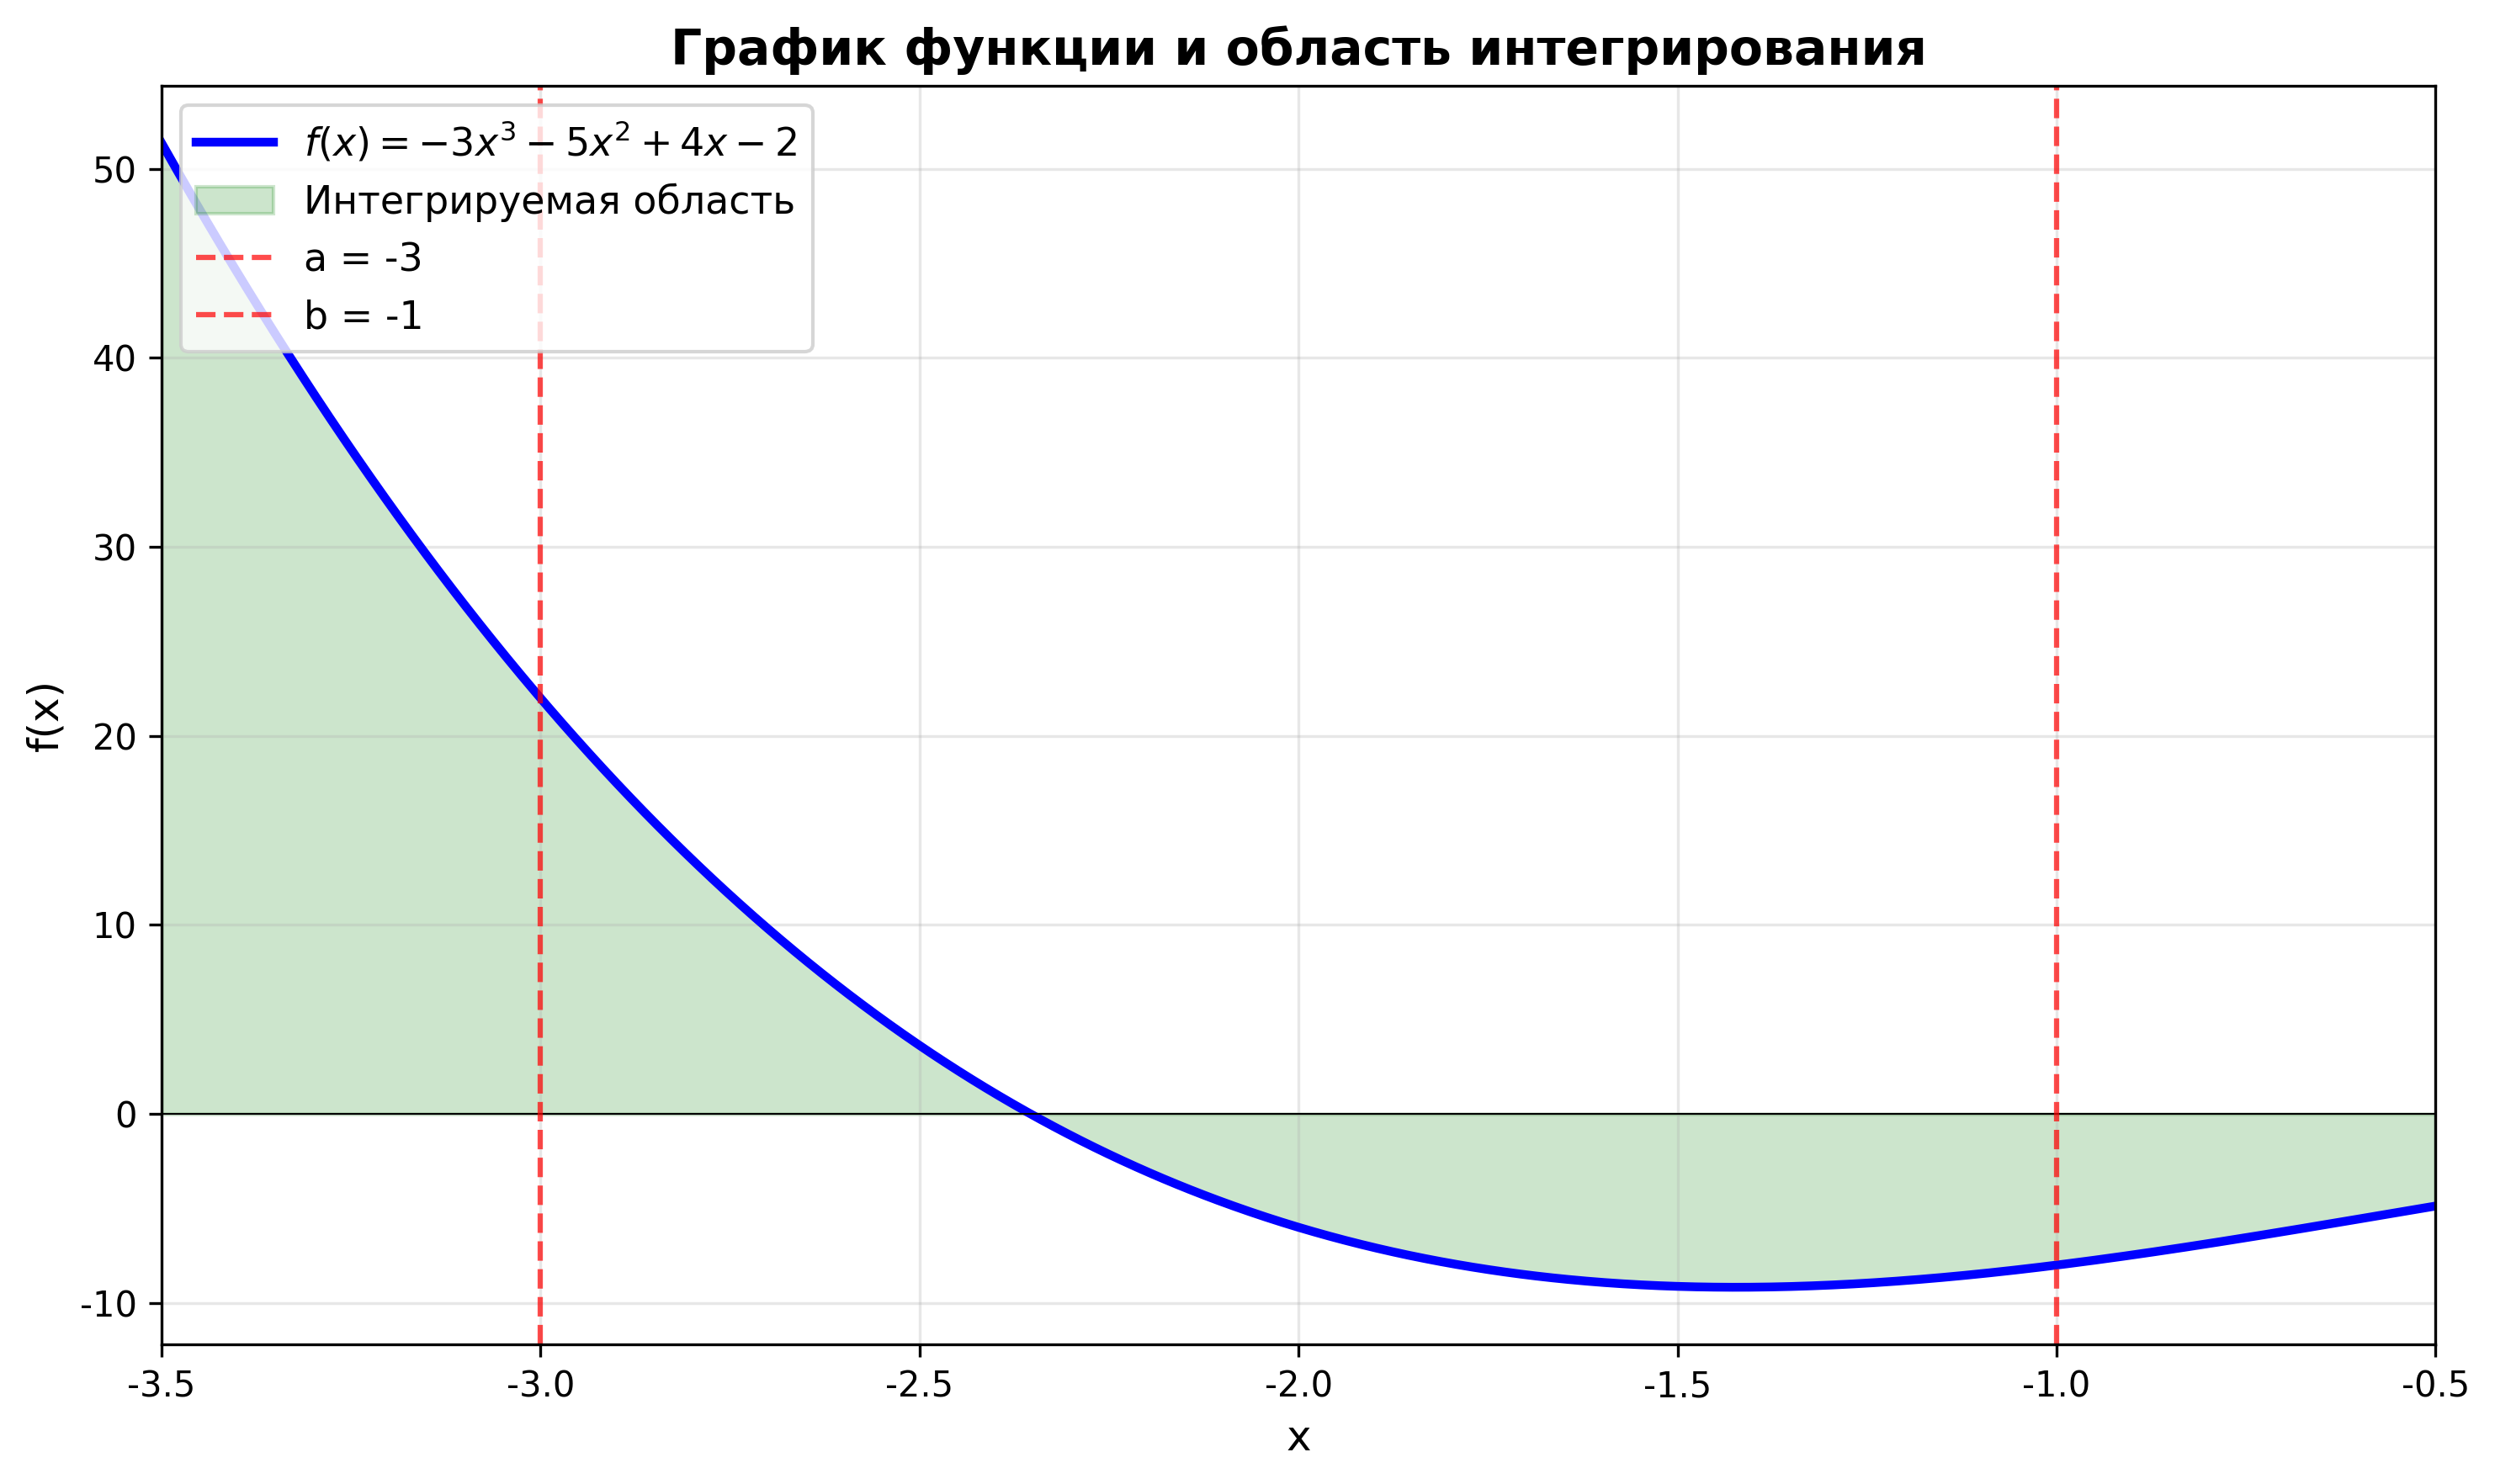
\includegraphics[width=0.82\linewidth]{plot_function}
    \caption{График функции и область интегрирования}
\end{figure}

\begin{figure}[h]
    \centering
    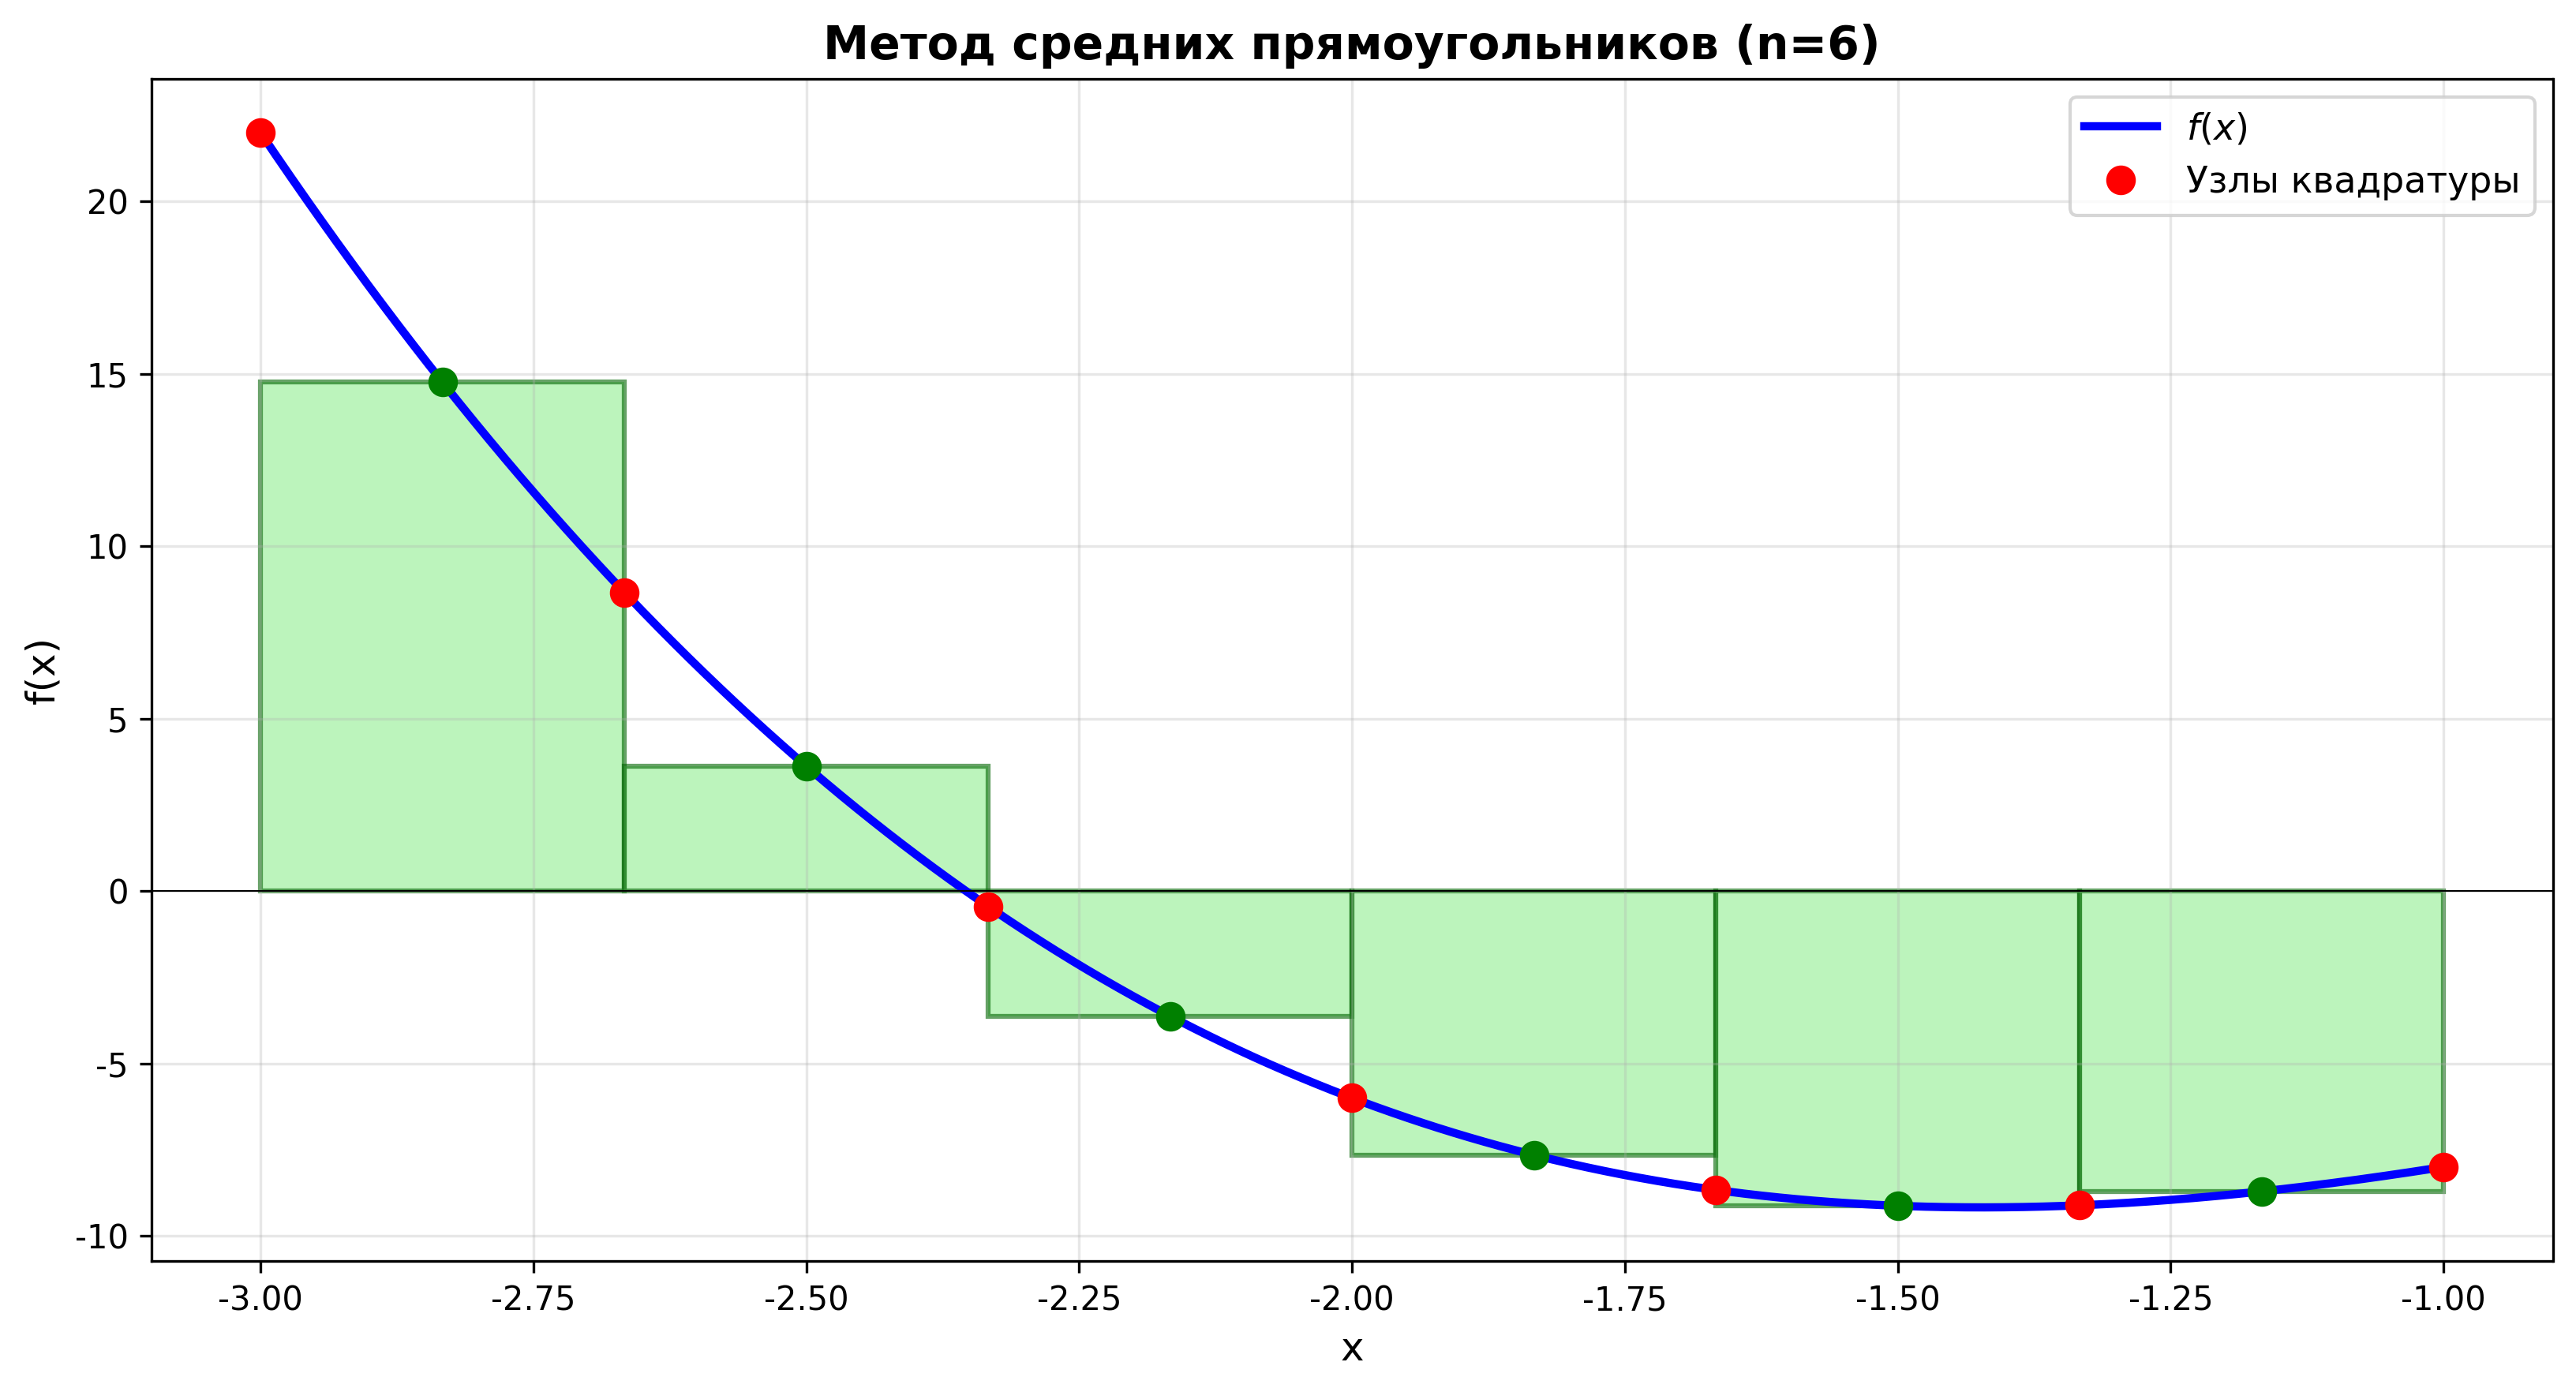
\includegraphics[width=0.82\linewidth]{plot_middle_rect}
    \caption{Метод средних прямоугольников ($n=6$)}
\end{figure}

\begin{figure}[h]
    \centering
    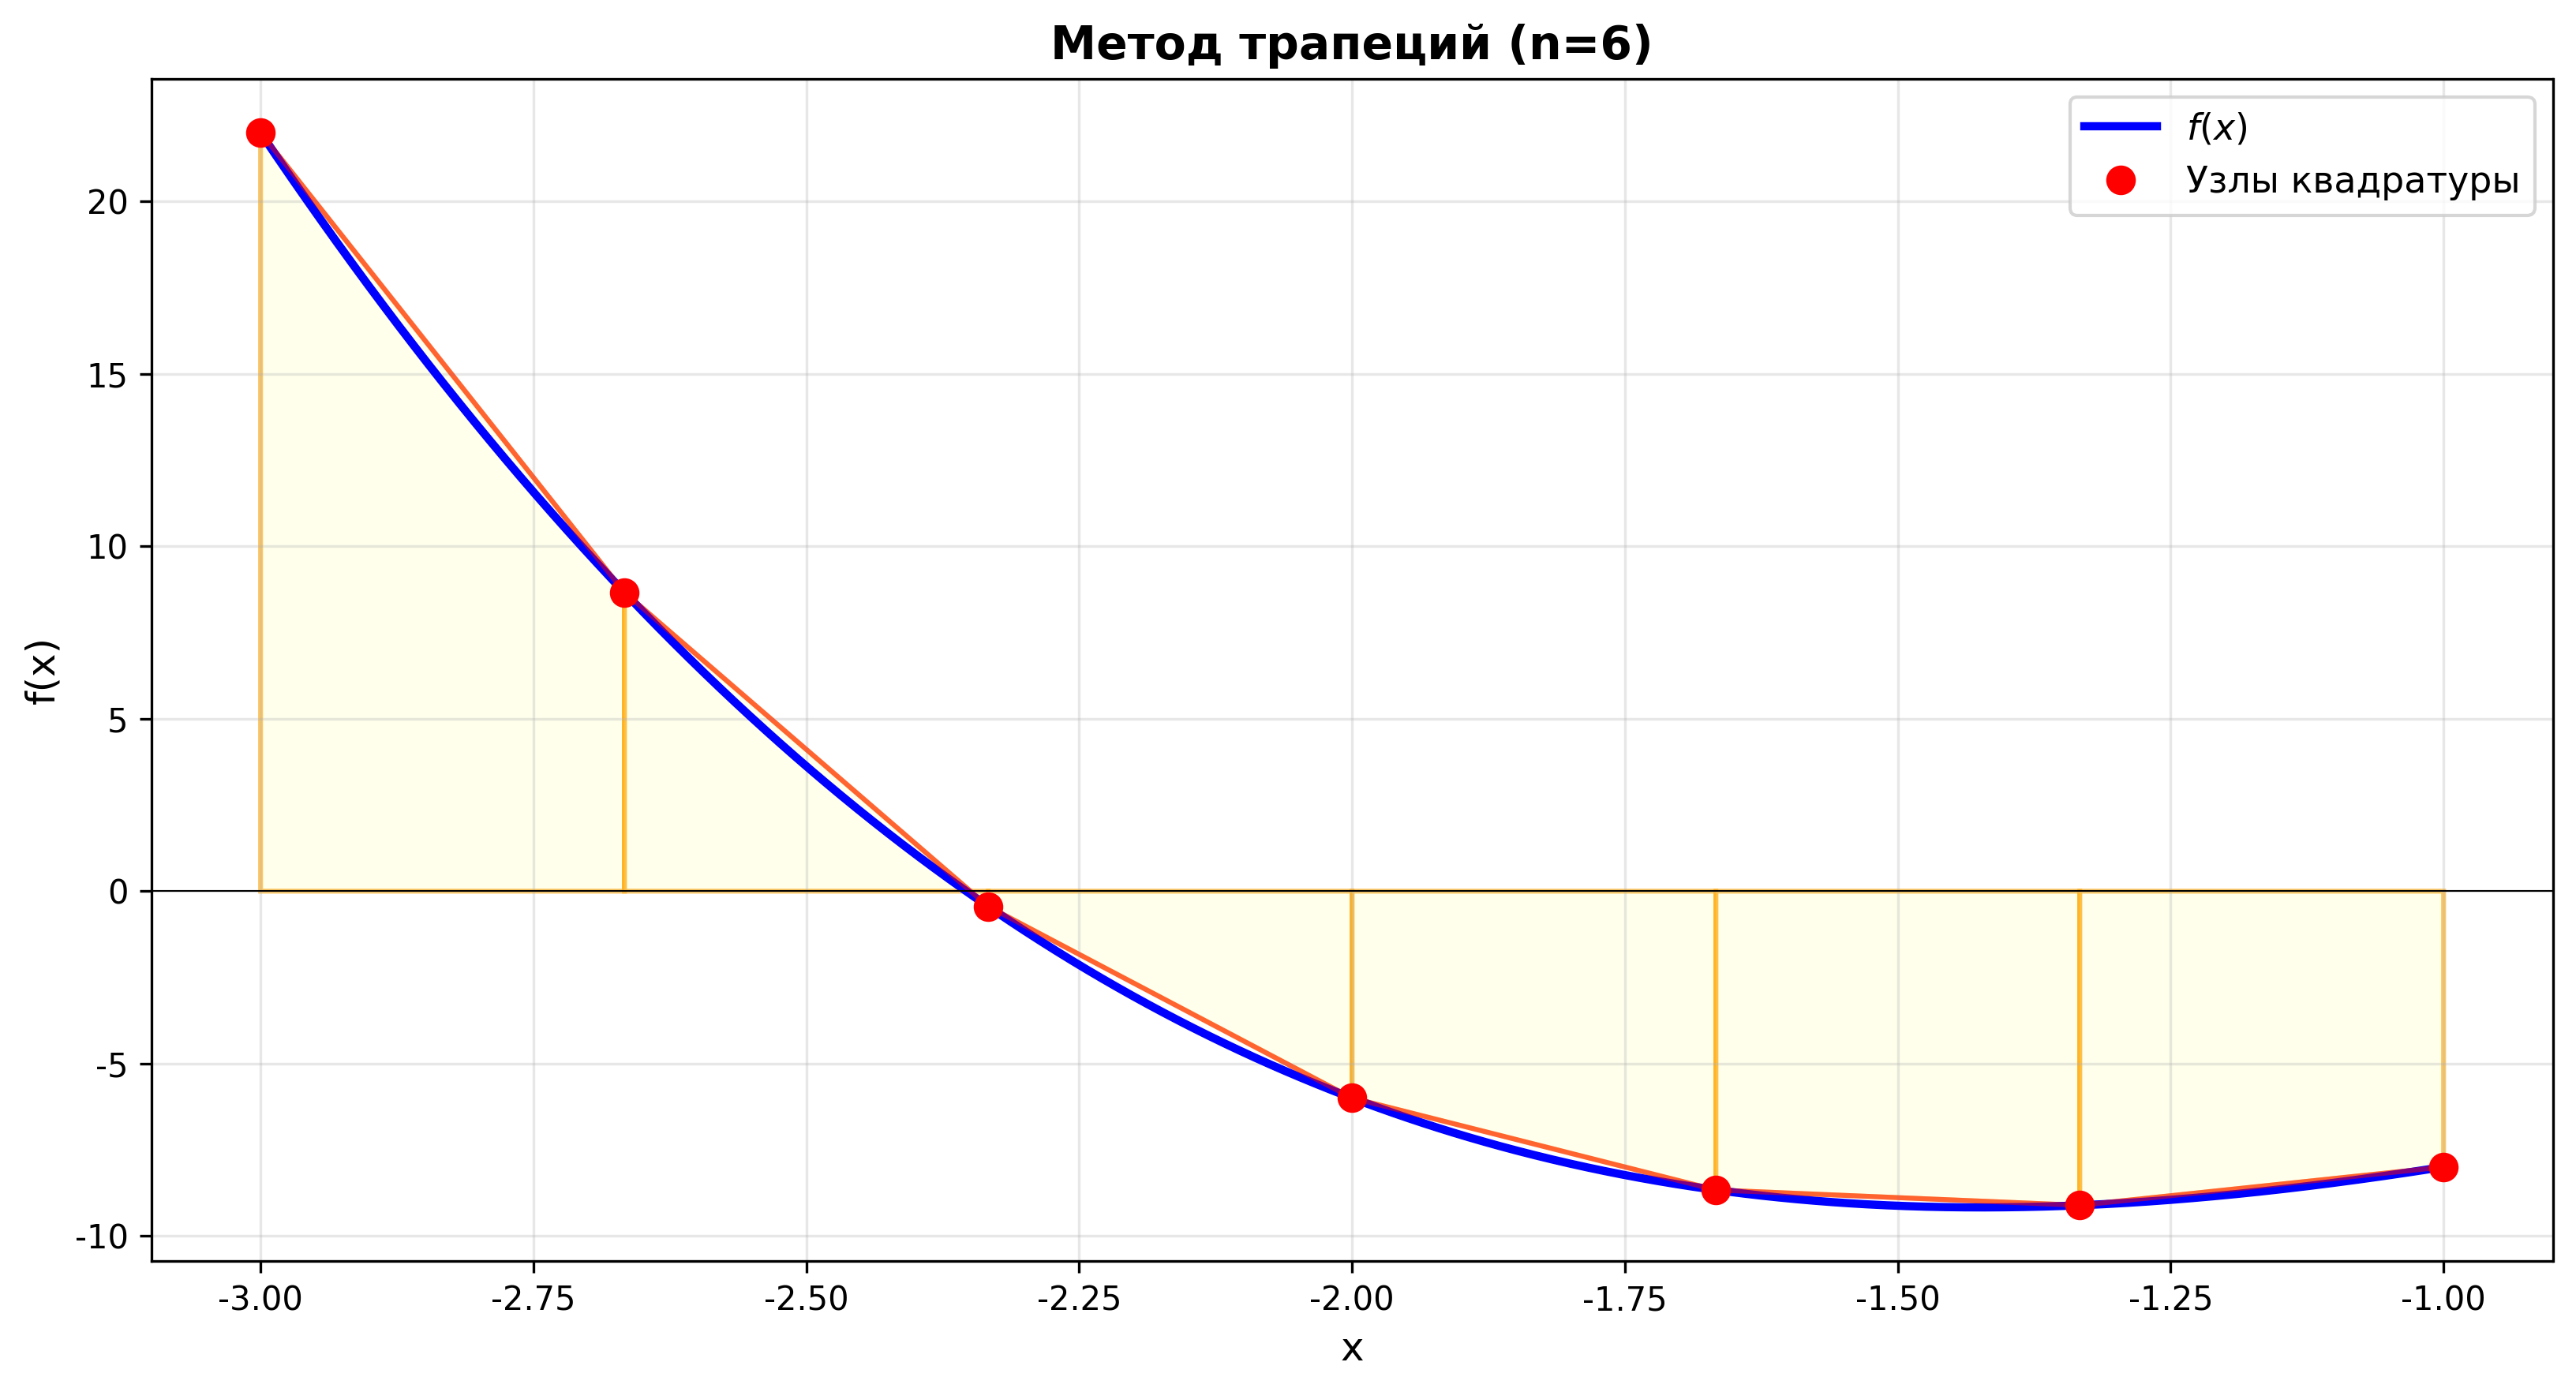
\includegraphics[width=0.82\linewidth]{plot_trapezoid}
    \caption{Метод трапеций ($n=6$)}
\end{figure}

\begin{figure}[H]
    \centering
    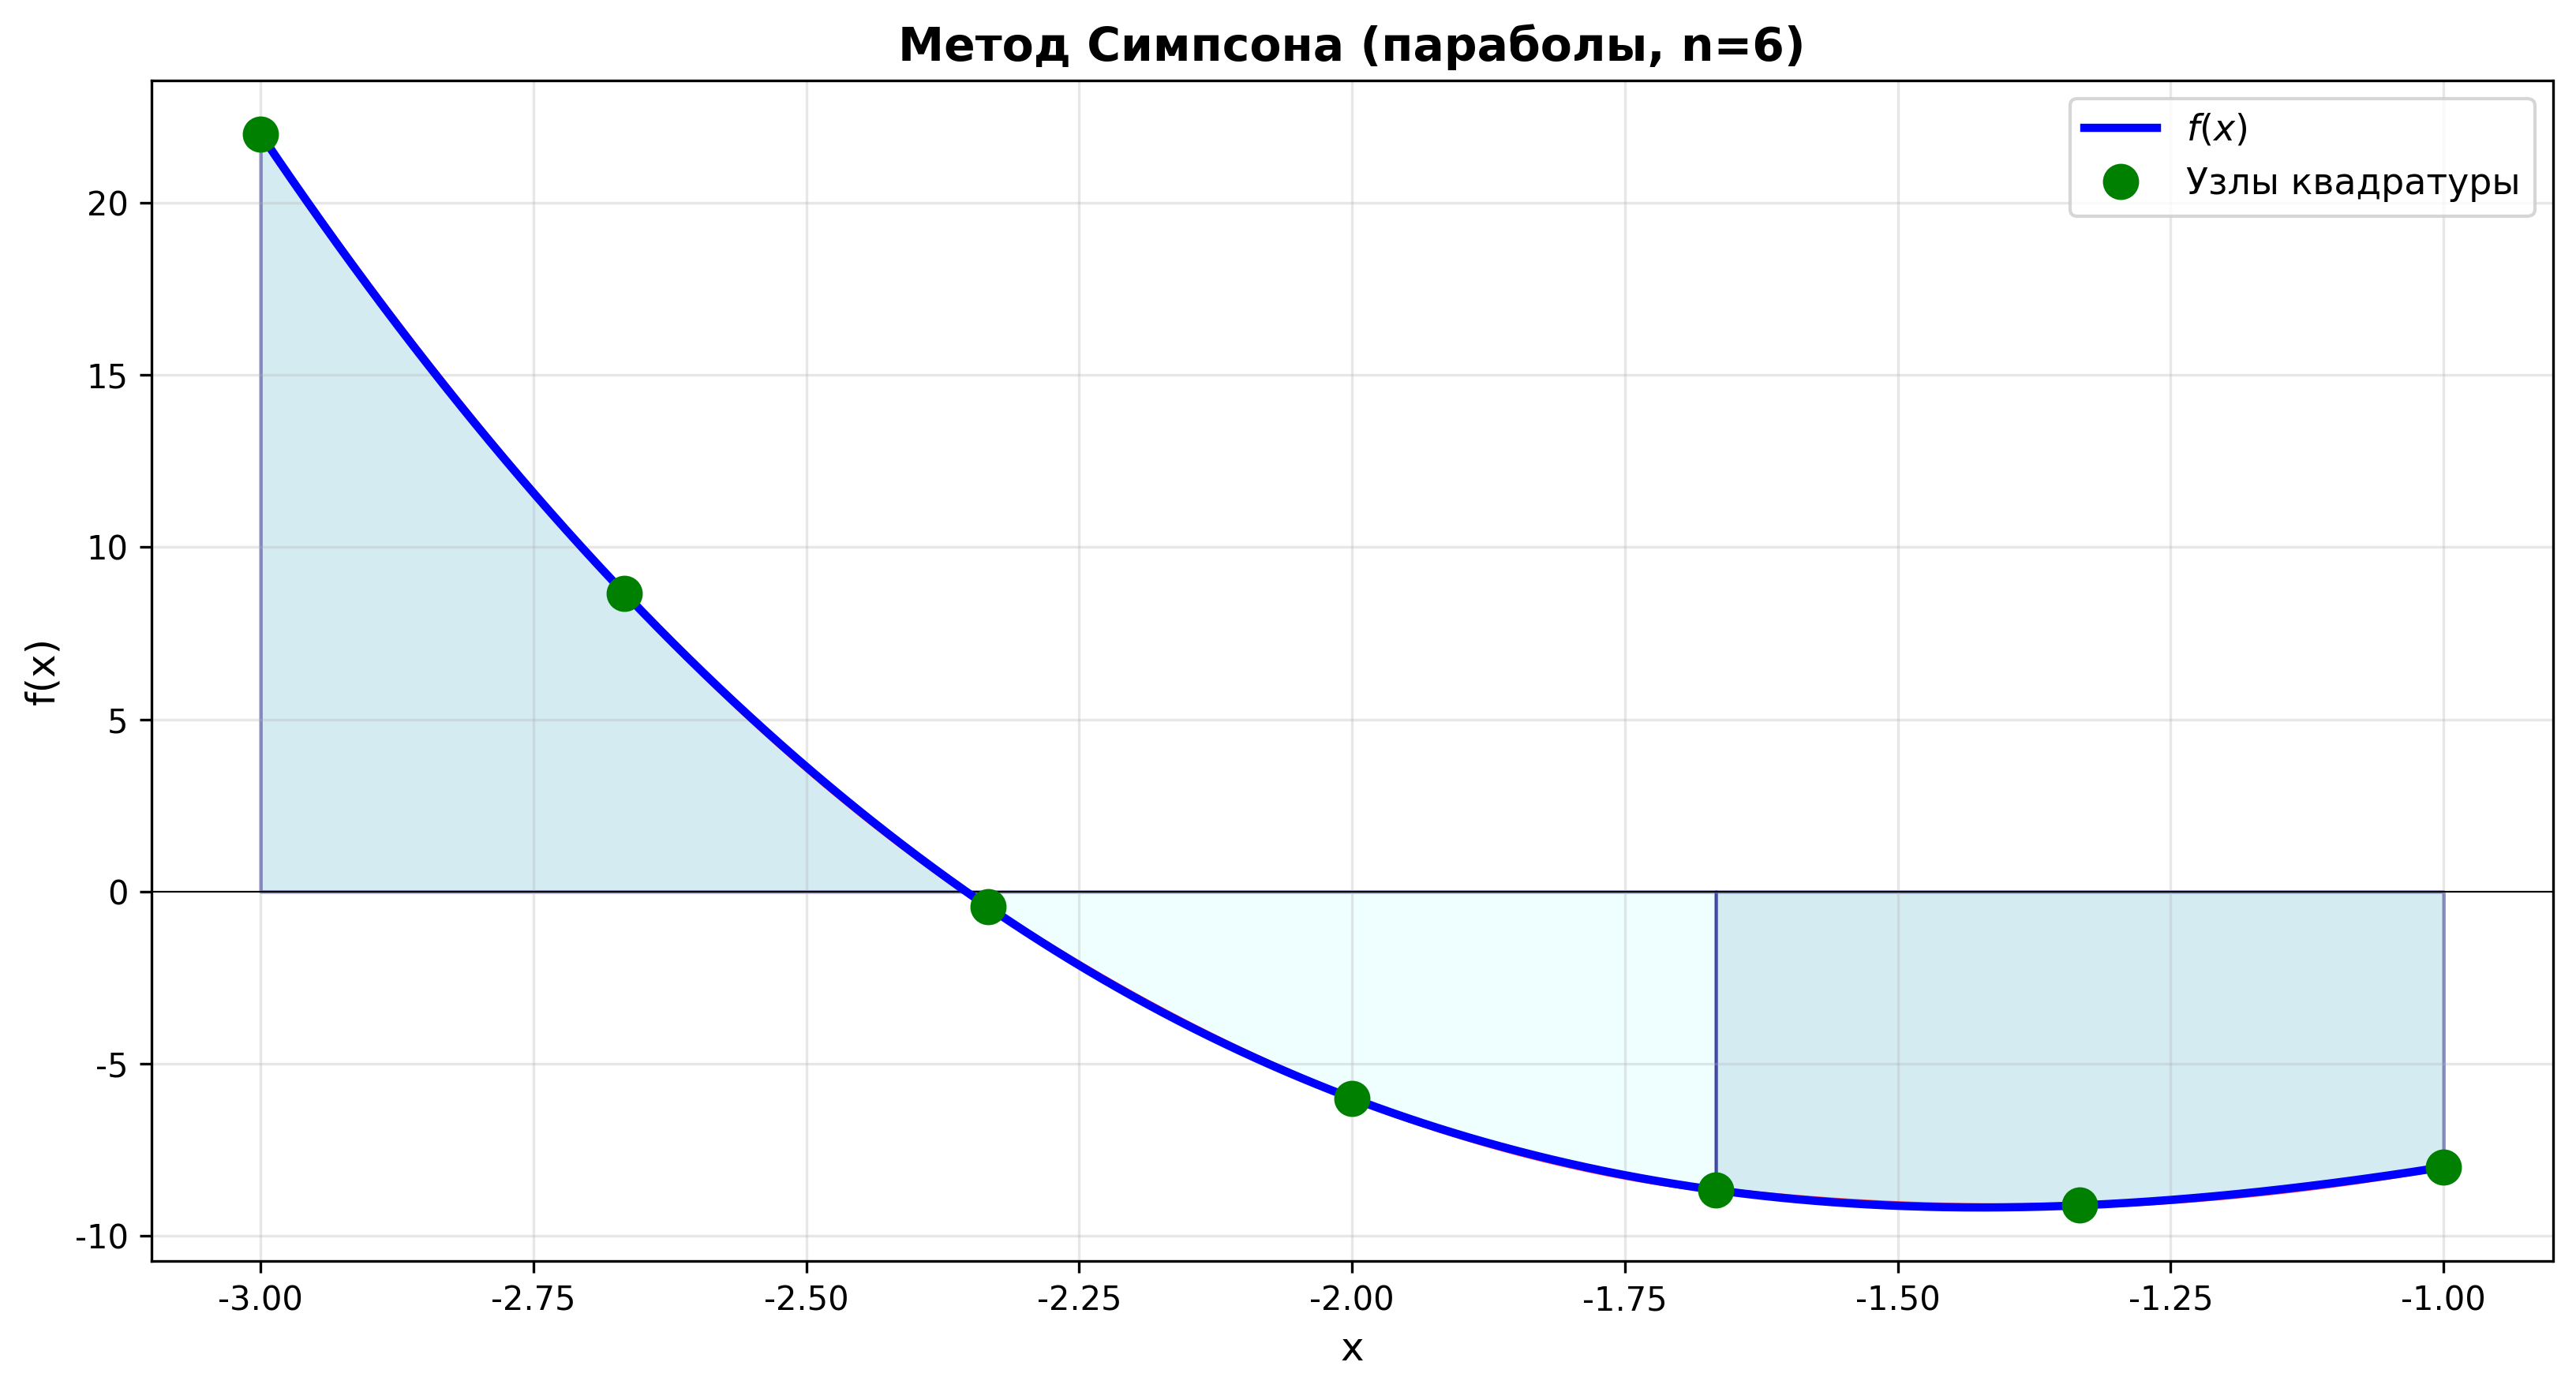
\includegraphics[width=0.82\linewidth]{plot_simpson}
    \caption{Метод Симпсона ($n=6$)}
\end{figure}
\newpage
\begin{figure}[H]
    \centering
    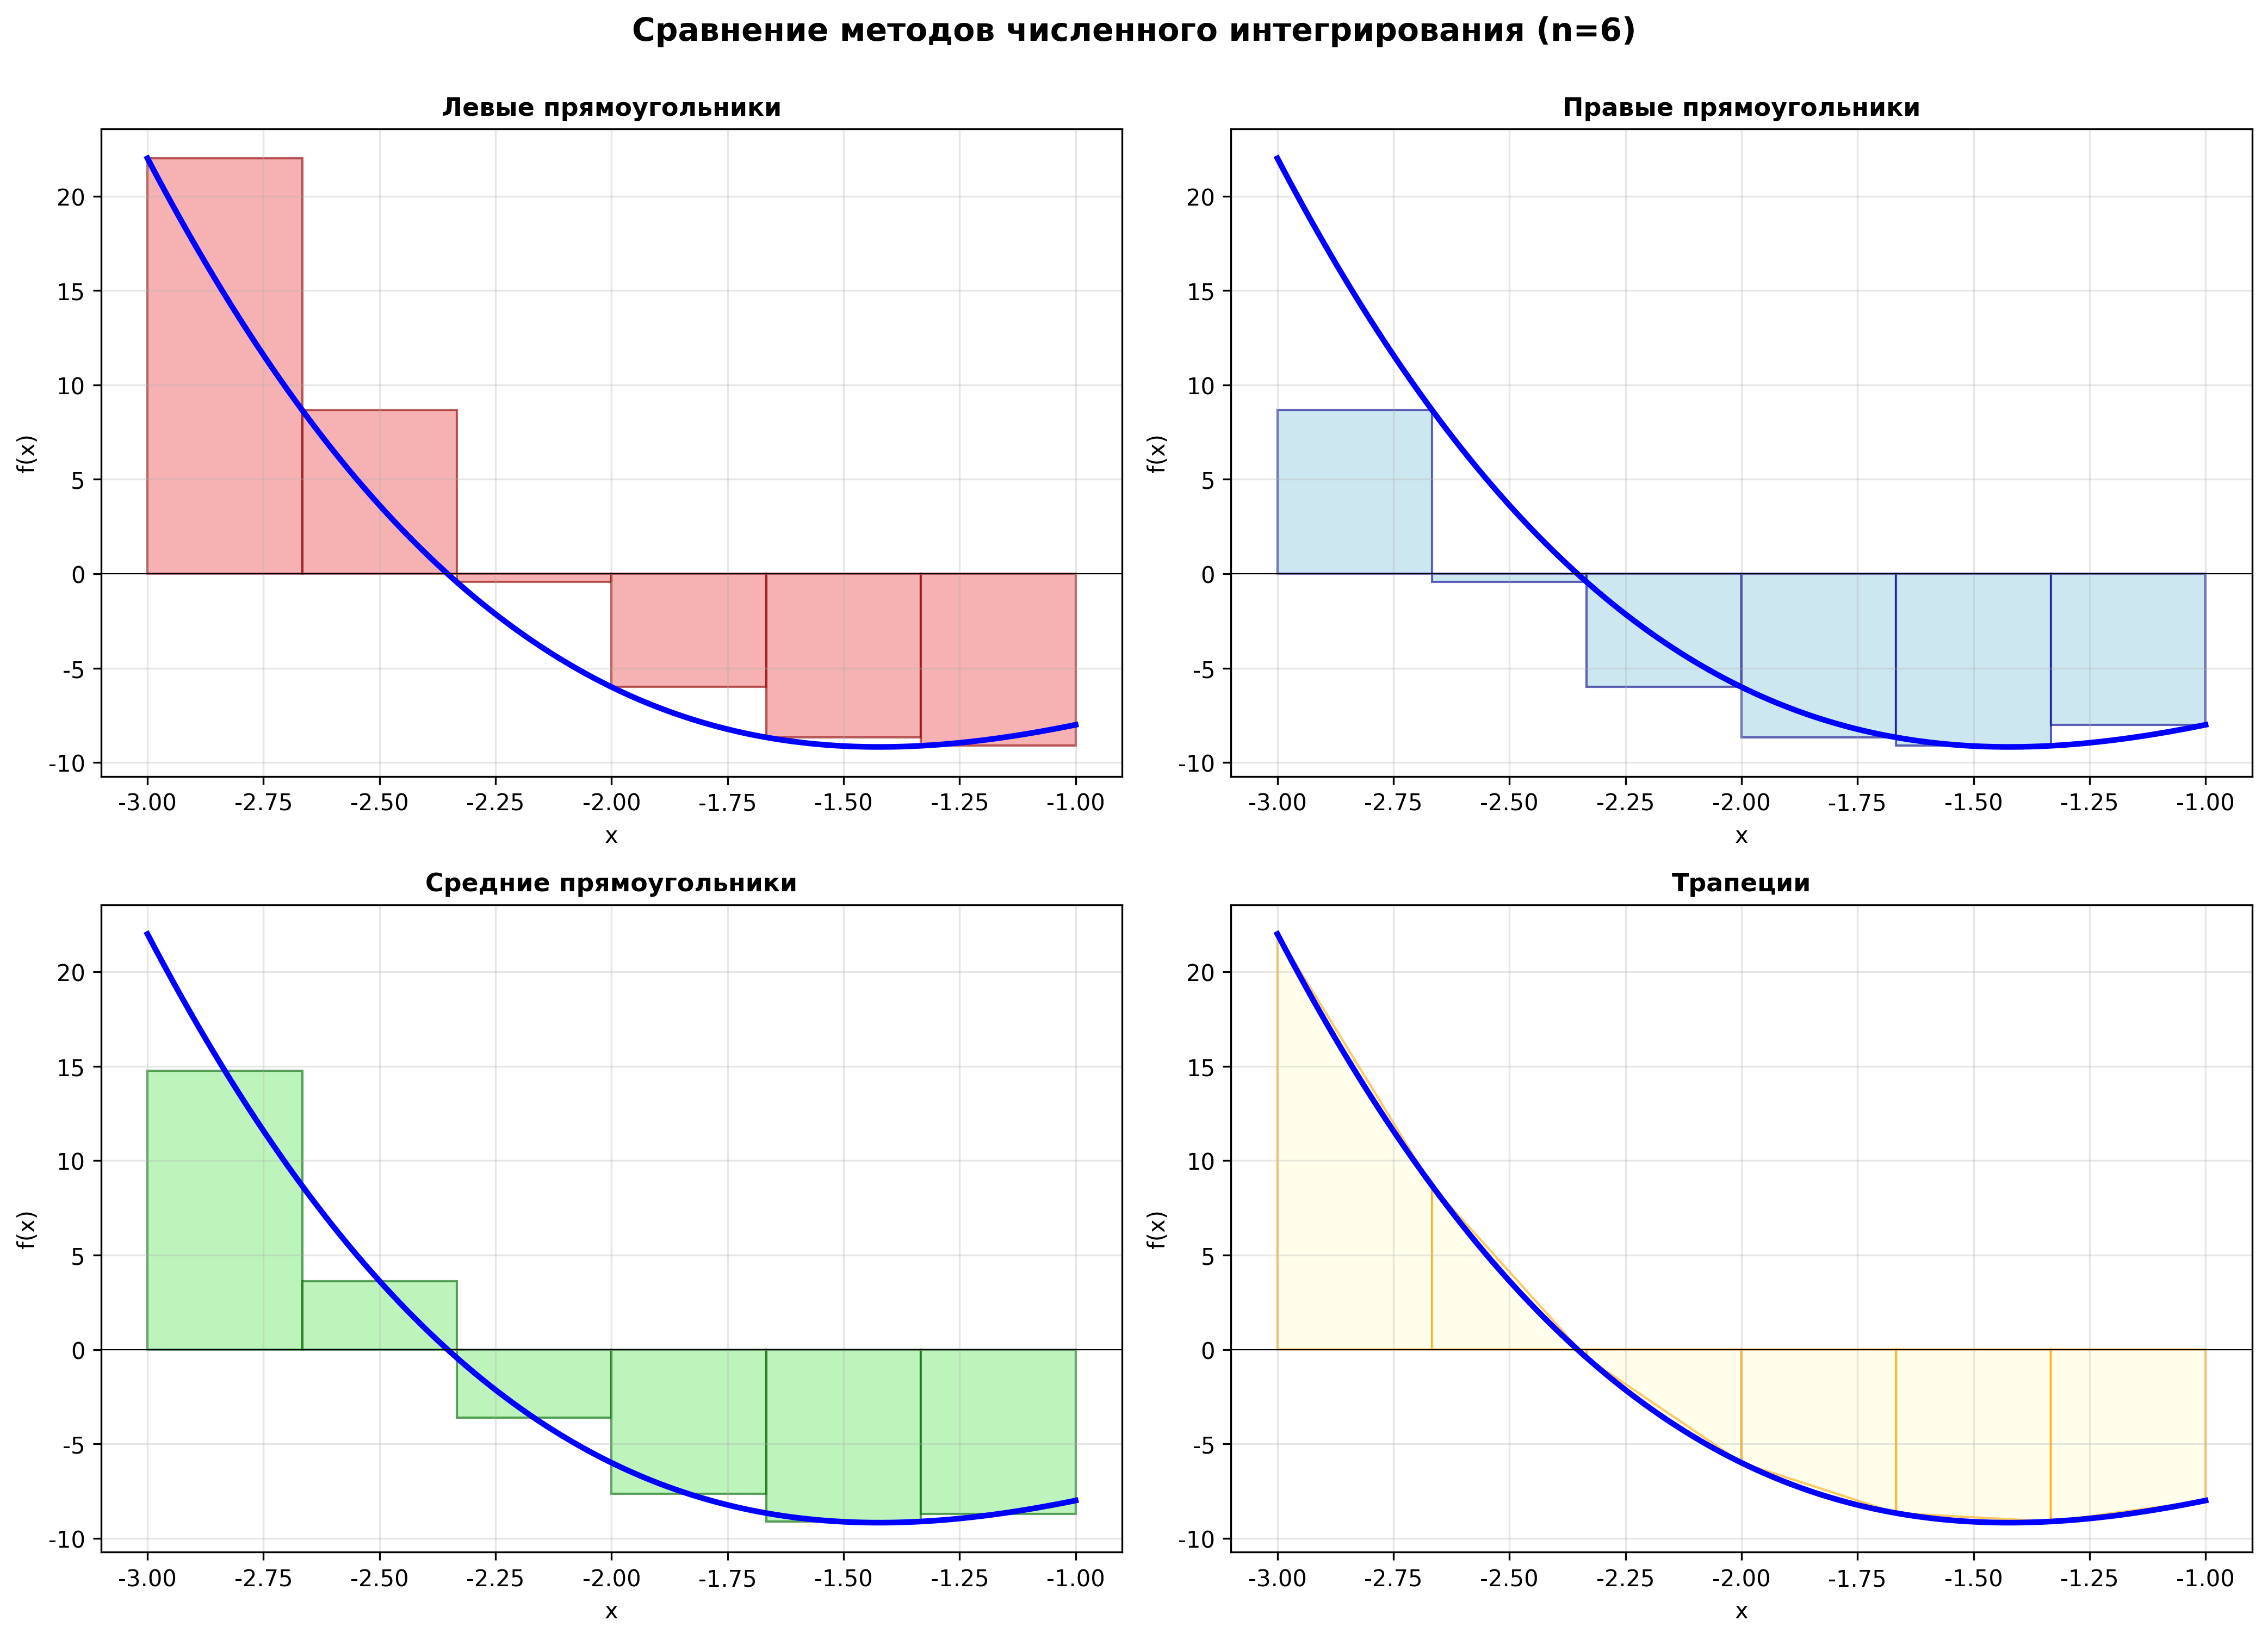
\includegraphics[width=0.82\linewidth]{plot_comparison}
    \caption{Сравнение методов численного интегрирования ($n=6$)}
\end{figure}


\newpage
\section{Программная реализация}

\subsection{Структура программы}

Программа разработана на Python 3 и реализует интерактивный интерфейс для численного интегрирования.

Основные компоненты:

\begin{enumerate}
    \item \textbf{Словарь VARIANTS} --- определение вариантов интегралов (функции, пределы, точные значения). Поддерживает 5 вариантов из таблицы задания.
    
    \item \textbf{Класс Integration} --- методы численного интегрирования:
    \begin{itemize}
        \item \texttt{left\_rect, right\_rect, middle\_rect} --- методы прямоугольников
        \item \texttt{trapezoid} --- метод трапеций
        \item \texttt{simpson} --- метод Симпсона
        \item \texttt{newton\_cotes\_6} --- формула Ньютона-Котеса
        \item \texttt{runge\_rule} --- оценка погрешности по правилу Рунге
    \end{itemize}
    
    \item \textbf{Класс Validator} --- валидация входных данных (выбор варианта, режима, точности с дефолтом 0.00001)
    
    \item \textbf{Класс App} --- интерактивное приложение с тремя режимами работы и бесконечным циклом выполнения
\end{enumerate}

\subsection{Реализованные вычислительные методы}



\begin{lstlisting}[style=intellij,caption={Левые прямоугольники}]
def left_rect(a: float, b: float, n: int, f: Callable) -> float:
    h = (b - a) / n
    return h * sum(f(a + i*h) for i in range(n))
\end{lstlisting}



\begin{lstlisting}[style=intellij,caption={Правые прямоугольники}]
def right_rect(a: float, b: float, n: int, f: Callable) -> float:
    h = (b - a) / n
    return h * sum(f(a + i*h) for i in range(1, n + 1))
\end{lstlisting}



\begin{lstlisting}[style=intellij,caption={Средние прямоугольники}]
def middle_rect(a: float, b: float, n: int, f: Callable) -> float:
    h = (b - a) / n
    return h * sum(f(a + (i + 0.5)*h) for i in range(n))
\end{lstlisting}



\begin{lstlisting}[style=intellij,caption={Метод трапеций}]
def trapezoid(a: float, b: float, n: int, f: Callable) -> float:
    h = (b - a) / n
    result = (f(a) + f(b)) / 2
    result += sum(f(a + i*h) for i in range(1, n))
    return h * result
\end{lstlisting}



\begin{lstlisting}[style=intellij,caption={Метод Симпсона}]
def simpson(a: float, b: float, n: int, f: Callable) -> float:
    if n % 2:
        n += 1
    h = (b - a) / n
    result = f(a) + f(b)
    result += 4 * sum(f(a + i*h) for i in range(1, n, 2))
    result += 2 * sum(f(a + i*h) for i in range(2, n, 2))
    return h/3 * result
\end{lstlisting}



\begin{lstlisting}[style=intellij,caption={Ньютона-Котеса n=6}]
def newton_cotes_6(a: float, b: float, f: Callable) -> float:
    n = 6
    h = (b - a) / n
    coeffs = [41, 216, 27, 272, 27, 216, 41]
    values = [f(a + i*h) for i in range(n + 1)]
    return (b - a) / 840 * sum(c * v for c, v in zip(coeffs, values))
\end{lstlisting}



\begin{lstlisting}[style=intellij,caption={Правило Рунге}]
def runge_rule(I_new: float, I_old: float, k: int) -> float:
    return abs(I_new - I_old) / (2**k - 1)
\end{lstlisting}


\subsection{Запуск программы}

\includegraphics[width=0.5\textwidth]{img.png}

\includegraphics[width=0.5\textwidth]{img_1.png}

\includegraphics[width=0.5\textwidth]{img_2.png}
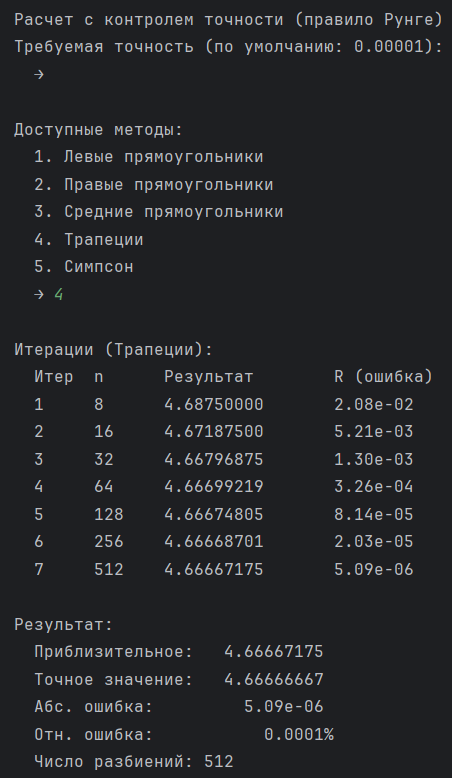
\includegraphics[width=0.5\textwidth]{img_3.png}
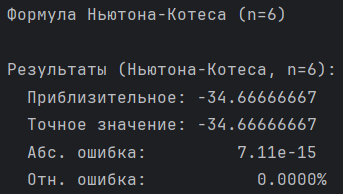
\includegraphics[width=0.5\textwidth]{img_4.png}


\newpage

% ─────────────────────────────────────────────────────────
\section{Выводы}

\subsection{Анализ численных методов интегрирования}

\subsubsection*{Точность методов}

\begin{itemize}
    \item \textbf{Методы 1-го порядка} (левые, правые прямоугольники): $O(h)$, низкая точность
    \item \textbf{Методы 2-го порядка} (средние прямоугольники, трапеции): $O(h^2)$, хорошая точность
    \item \textbf{Методы 4-го порядка} (Симпсон, Ньютона-Котеса): $O(h^4)$ --- $O(h^8)$, высокая точность
\end{itemize}

\subsubsection*{Скорость сходимости}

Для одной и той же точности требуется число разбиений:
\begin{center}
\begin{tabular}{|l|c|}
\hline
\textbf{Метод} & \textbf{Порядок аппроксимации} \\
\hline
Левые/Правые прямоугольники & $O(h)$ \\
Средние прямоугольники & $O(h^2)$ \\
Трапеции & $O(h^2)$ \\
Симпсон & $O(h^4)$ \\
Ньютона-Котеса (6-й) & $O(h^8)$ \\
\hline
\end{tabular}
\end{center}

\subsubsection*{Практические рекомендации}

\begin{enumerate}
    \item Используйте \textbf{метод Симпсона} как основной универсальный метод

    \item Применяйте \textbf{правило Рунге} для автоматического выбора числа разбиений

    \item Для \textbf{гладких функций} используйте формулы высокого порядка (Ньютона-Котеса)

    \item Всегда \textbf{проверяйте сходимость} и оценивайте погрешность

    \item Для \textbf{несобственных интегралов} применяйте специальные техники
\end{enumerate}

\subsection{Итоги выполнения лабораторной работы}

\begin{itemize}
    \item ✓ Вычислено \textbf{точное значение интеграла} аналитически: $I = -\frac{10}{3} \approx -3.33333$

    \item ✓ Применена \textbf{формула Ньютона-Котеса} 6-го порядка: получена точность машинного нуля

    \item ✓ Вычислены значения по \textbf{методам среднихпрямоугольников, трапеций и Симпсона} при n=10

    \item ✓ Применено \textbf{правило Рунге} для оценки погрешности и контроля точности

    \item ✓ Реализованы все методы в виде отдельных функций класса Integration

    \item ✓ Проведено \textbf{сравнение точности методов}:
    \begin{itemize}
        \item Симпсон: точность $\sim 10^{-15}$ (машинный нуль)
        \item Ньютона-Котеса: точность $\sim 10^{-15}$ (машинный нуль)
        \item Средние прямоугольники: ошибка $2.6\%$ при n=10
        \item Трапеции: ошибка $5.2\%$ при n=10
    \end{itemize}

    \item ✓ Создана \textbf{интерактивная программа} с тремя режимами работы

    \item ✓ Все результаты \textbf{совпадают с теоретическими предсказаниями}
\end{itemize}

\subsection{Заключение}

Метод Симпсона и формулы Ньютона-Котеса высокого порядка показали исключительную точность для полиномов. Правило Рунге позволяет автоматически выбирать число разбиений для достижения требуемой точности. Реализованная программа демонстрирует практическое применение численного интегрирования и может быть использована для вычисления интегралов от произвольных функций.

\end{document}
